\documentclass[twoside, 12pt]{report}
\usepackage[utf8]{inputenc}
\usepackage{abstract,lipsum}
\usepackage[english]{babel}
\usepackage{geometry}
 \geometry{
 a4paper,
 total={160mm,247mm},
 left=30mm,
 top=30mm,
 asymmetric
 }
\usepackage{graphicx}
\usepackage{eso-pic}
\usepackage{color, xcolor, colortbl}
\usepackage{enumitem}
\usepackage{dsfont}
\usepackage{ragged2e}
\usepackage{makecell}
\usepackage{fancyhdr}
\usepackage[nottoc, notlof, notlot,numbib]{tocbibind}
\usepackage{caption}
\usepackage{subcaption}
\usepackage{hyperref}
\usepackage{booktabs}
\usepackage{amsmath, amsfonts, amssymb,amsthm}
\usepackage{algorithm,algpseudocode}
\usepackage{graphicx} % Allows including images
\usepackage{booktabs} % Allows the use of \toprule, \midrule and \bottomrule in tables
\usepackage{float}
\usepackage{appendix}
\usepackage{svg}
\usepackage{listings}
\usepackage{sectsty}
\usepackage{setspace}
\usepackage{slantsc}
\usepackage{url}
\usepackage{titlesec}
\lstset { %
    language=python, % set backgroundcolor
    basicstyle=\footnotesize,% basic font setting
}

\newcommand{\mycode}{                               % Name after the Language used
    \lstset{
        basicstyle=\ttfamily\small,                 % Code Font Size
        keywordstyle=\color{darkpurple}\bfseries,   % Color Key Word
        stringstyle=\color{darkblue},               % Color String
        identifierstyle=\color{teal},
        commentstyle=\color{darkgreen},             % Color Comment
        morecomment=[s][\color{blue}]{/**}{*/},     % Color Comment
        tabsize=2,                                  % Tab Size
        captionpos=b,                               % Caption Position
        showtabs=false,                             % Show Tabs within Strings
        showspaces=false,                           % Show Spaces Code
        showstringspaces=false,                     % Show Spaces Strings
        stepnumber=1,                               % Line Number Step
        numbers=left,                               % Line Number Position
        numbersep=5pt,                              % Line Number Distance from Code
        numberstyle=\tiny\color{gray},              % Line Number Style
        frame=single,                               % Frame
        rulecolor=\color{black},                    % Frame Color
        xleftmargin=10pt,                            % Left Margin
        backgroundcolor=\color{white},              % Background Color
        breaklines=true,                            % Break Automatic Line
        breakatwhitespace=true,                     % Break Automatic Spaces 
        breakautoindent=false,                      % Break Automatic Indent
        extendedchars=true,                         % 
        inputencoding=latin1,                       % Encoding
        literate=                                   % Including Especial Charects To Write in French
                {é}{{\'{e}}}1
                {è}{{\`{e}}}1
                {ê}{{\^{e}}}1
                {ë}{{\¨{e}}}1
                {É}{{\'{E}}}1
                {Ê}{{\^{E}}}1
                {û}{{\^{u}}}1
                {ù}{{\`{u}}}1
                {ú}{{\'{u}}}1
                {â}{{\^{a}}}1
                {à}{{\`{a}}}1
                {á}{{\'{a}}}1
                {ã}{{\~{a}}}1
                {ä}{{\"{a}}}1
                {Á}{{\'{A}}}1
                {Â}{{\^{A}}}1
                {Ã}{{\~{A}}}1
                {Ä}{{\"{A}}}1
                {ç}{{\c{c}}}1
                {Ç}{{\c{C}}}1
                {õ}{{\~{o}}}1
                {ó}{{\'{o}}}1
                {ô}{{\^{o}}}1
                {ö}{{\"{o}}}1
                {Õ}{{\~{O}}}1
                {Ó}{{\'{O}}}1
                {Ô}{{\^{O}}}1
                {Ö}{{\"{O}}}1
                {î}{{\^{i}}}1
                {Î}{{\^{I}}}1
                {í}{{\'{i}}}1
                {Í}{{\~{Í}}}1
                {ü}{{\"{u}}}1
                {Ü}{{\"{U}}}1
    }
}

%\usepackage[alf,bibjustif,abnt-etal-cite=3,abnt-etal-list=0,abnt-repeated-author-omit=yes]{abntex2cite}
%\bibliographystyle{abntex2-alf}

\makeatletter
\renewenvironment{titlepage}
 {%
  \if@twocolumn
    \@restonecoltrue\onecolumn
  \else
    \@restonecolfalse\newpage
  \fi
  \thispagestyle{plain}%
 }
 {%
  \if@restonecol
    \twocolumn
  \else
    \newpage
  \fi
 }
\makeatother

\providecommand{\keywords}[1]
{
  \small	
  \textbf{\textit{Keywords---}} #1
}

\newcommand{\source}[1]{\caption*{Source: {#1}} }

\renewcommand{\indent}[1]{\setlength{\parindent}{#1}}
\DeclareMathOperator{\spn}{span}
\newcommand{\sepline}{\vspace{-1mm} \line(1,0){60} \vspace{-1mm}}
\newcommand{\norm}[1]{\left\lVert#1\right\rVert}

%\title{Projet de Recherche (PRe}
\author{nomenome}
\date{May 2024}

% -----------------------------------------------------------------
% Top and bottom of the pages are set here
% -----------------------------------------------------------------
\pagestyle{fancy}
\fancyhf{}
\fancyhead[CO]{} % FIXME: fill this?
\fancyhead[CE]{\rightmark}
\cfoot{GUIMARAES Eduardo - POEMS Laboratory \break \color{red} This work is non confidential}
\rfoot{\thepage}

\begin{document}

% -------------------------------------------
% Title Page
% -------------------------------------------

\begin{titlepage}
  \thispagestyle{empty}

  \begin{figure}[h]
    \centering
    \begin{minipage}[b]{0.45\textwidth}
      \raggedright
      \includesvg[height=0.4\textwidth]{images/ensta_logo.svg}
    \end{minipage}
    \hfill
    \begin{minipage}[b]{0.4\textwidth}
      \raggedleft
      \includesvg[height=0.4\textwidth]{images/poems_logo.svg}
    \end{minipage}
  \end{figure}

  \vfill

  \centering{\LARGE \textbf{Research Internship (PRe)}} \\
  \hfill\\
  \centering{\large \textbf{Field of Study: Applied Maths}}\\
  \centering{\large \textbf{Scholar Year : 2023-2024}} \\
  \hfill\\
  \vfill
  \centering{\huge \textbf{Hierarchical Matrices and \\ Inexact GMRES}}
  \vfill
  \color{red} \noindent  \fbox{%
    \parbox{\textwidth}{%
      \centering{\LARGE \textbf{Confidentiality Notice}}\\
      \centering{\normalsize Non-confidential and publishable report}
    }%
  }
  \vfill
  \color{black}
  \large \textbf{Author: GUIMARAES Eduardo \hfill Promotion: 2025}\\
  \vspace{5mm}
  \FlushLeft{\normalsize \textbf{
      \begin{tabular}{rl}
        ENSTA Paris Tutor: & FARIAS Luiz \\ &MARCHAND Pierre
      \end{tabular}
    }} \\
  \normalsize \textbf{Host Organism Tutor: CHAPOUTOT Alexandre}

  \vfill
  \centering{\normalsize \textbf{Internship from 13/05/2024 to 15/08/2024}} \\
  \vspace{1cm}
  \centering{\normalsize \textbf{POEMS}} \\
  \centering{\normalsize \textbf{Address: 828, Boulevard des Maréchaux, 91762 Palaiseau France}}
\end{titlepage}


% -------------------------------------------
% Blank page (?)
% -------------------------------------------
\section*{}
\vfill
\paragraph{}
\begin{center}
  This page was intentionally left blank.
\end{center}
\vfill

% -------------------------------------------
% Confidentialy Notice
% -------------------------------------------
\newpage

\section*{Confidentiality Notice}
\vfill
\paragraph{}
This present document is not confidential. It can be communicated outside in paper format
or distributed in electronic format.
\vfill

% -------------------------------------------------------------------
% Writing part
% -------------------------------------------------------------------


\begin{abstract}
    In this project we will focus on combining a recently develop inexact GMRES algorithm, which differs from the classic
    GMRES algorithm in that the underlying linear system is allowed to change at each iteration, and hierarchical matrix
    approximation to a boundary integral discretisation. The main goal is to (i) understand the inner workings of GMRES
    and how changing the linear system at each iteration affects the convergence properties, and (ii) explore whether
    inexact GMRES has practical interest when combined with a variable precision
    $\mathcal{H}$-matrix compression. This project
    % FIXME: "will be carried out" or "was carried out"?
    will be carried out in the context of two existing libraries:
    \href{https://github.com/IntegralEquations/HMatrices.jl}{HMatrices.jl} and
    \href{https://github.com/IntegralEquations/Inti.jl}{Inti.jl}. The internship
    % FIXME: is the future tense correct?
    will take place at the POEMS laboratory, and will be supervised by Luiz M. Faria (chercheur INRIA) and Pierre
    Marchand (chercheur INRIA).
\end{abstract} \hspace{10pt}

\keywords{GMRES, BEM, applied maths, acceleration, Julia}


\section*{Acknowledgments}
\paragraph{}

I am deeply grateful to all those who have contributed to the successful completion of this research project during my internship at UMA and the POEMS group.

First and foremost, I would like to express my sincere gratitude to Mr. Farias and Mr. Marchand for providing me with this opportunity. The guidance provided during the project allowed me to work in a field that interests me very much and that I intend to pursue after my stay at ENSTA Paris. I also extend this gratitude for ENSTA Paris and UMA, who granted the funding of the project and made everything possible.

I would also like to extend my heartfelt thanks all students and staff of UMA that I have had the opportunity of meeting and/or working with. Even though I'm far away from home, the environment they created always made me feel welcomed and thankful for the support I received. A special mention goes to the students I had the pleasure of sharing a room with, and whose company helped shape this amazing experience.

Finally, I wish to thank my family and friends, both at Brazil but also the ones I got to meet here in France and are already considered as a part of my family. 

Thank you all for your invaluable contributions to this research.

\newpage
\tableofcontents

\newpage
\listoffigures

\fancyhead[CE]{\leftmark}

%\newpage
\chapter{Iterative Methods and Krylov's Subspace}
\section{Iterative Methods and motivation}

We consider the solution of a linear system, with $A \in \mathbb{C}^{n \times n}$ an invertible matrix with elements in \gls{complex}, $b \in \mathbb{C}^{n}$ our right-hand side and $x\in \mathbb{C}^{n}$ a vector of unknowns:

\begin{equation}\label{eq:linear_systinit}
    Ax=b
\end{equation}


A system that can be solved by direct methods, like \textit{Gaussian elimination} and \textit{LU decomposition}. The problem with such approaches comes with their complexity: direct methods usually have $\mathcal{O}(m^{3})$ complexity \cite{trefethen1998numerical}, where $m$ is the dimension of the input matrix. Since we apply larger matrices in practice, to achieve high resolution in the solution of a \acrshort{pde}, the direct algorithms become too slow, and we require a more efficient approach.


These iterable methods find, after a certain number of iterations, a sequence ${x_{k}}$ that converges to $x$, the exact solution of the problem \ref{eq:linear_systinit}. This should be done while making the large-scale computations faster, i.e., obtaining a complexity smaller than $\mathcal{O}(m^{3})$, and keeping a maximum tolerance between the iterable solution and the exact one.


\begin{equation}\label{eq:suite}
    x = \lim_{k \to \infty} x_{k}
\end{equation}


The method stops after $k$ iterations, where $x_{k}$ is the fist element of the sequence to satisfy the condition \ref{eq:residual}.

\begin{equation}\label{eq:residual}
    \frac{||Ax_{k} - b||}{||b||} \leq \epsilon
\end{equation}

We define $\epsilon$ as the tolerance given to the algorithm.

To achieve a smaller complexity than $\mathcal{O}(m^{3})$, Iterative Methods employ matrix vector products, complexity $\mathcal{O}(m^{2})$, instead of the product between matrices found in direct methods. So, considering an Iterative Method finds a solution in $k$ steps, its complexity would be $\mathcal{O}(km^{2})$.

Therefore, if $k<<m$, i.e., the number of iterations is sufficiently smaller than $m$, the iterative methods become more efficient than the direct ones.



The method we employ in our problems is the \acrfull{gmres}, explained later in the report. Its main idea involves the projection of a high dimensional problem, as large as $A$ in \ref{eq:residual}, in a lower dimensional \textit{Krylov Space}:

\begin{equation}\label{eq:xkry}
    x_{k} \in \spn(b,Ab,A^{2}b,...,A^{k-1}b)
\end{equation}

Explained in more detail below.

\section{Krylov subspace}
Let $A \in \mathbb{C}^{n \times n}$ a matrix and $b\in \mathbb{C}^{n}$. For each $k\leq n$ the Krylov subspace $\mathcal{K}_{k}=\mathcal{K}_{k}(A,b)$ associated to A, b is defined as \ref{eq:krylov}.

\begin{equation}\label{eq:krylov}
    \mathcal{K}_{k}(A,b) = \spn(b,Ab,A^{2}b,\dots , A^{k-1}b)
\end{equation}

These subspaces also have the following property: $k<l \to \mathcal{K}^{k} \subset \mathcal{K}^{l}$ \cite{bonnet}.

The subspace $\mathcal{K}_{k}(A,b)$ is also the subspace of all the vectors from $\mathbb{R}^{m}$ which could be written as $x=p(A)b$, where $p(A)$ is a polynomial of degree less than $k-1$ which $p(0)=1$.

The problem with using ${A^{k}b}, k \in {0,1,2,\dots}$ as a base comes from the fact that successive products of $A$ make vectors that are \textit{approximately collinear}, since those are really close of the eigenvector with the largest eigenvalue of $A$.

Such problem then requires finding a new base for this space, one that does not suffer from the power iteration of $A$, and it is the subject of the next section.

\section{Arnoldi's Method}


Arnoldi's Method is an orthogonal projection method used to find an orthonormal basis ${q_{1}, \dots, q_{k}}$ to $\mathcal{K}_{k}(A,b)$.

An algorithm for the method can be found in \ref{alg:arnoldi}.


\begin{algorithm}
    \caption{Arnoldi's iteration}\label{alg:arnoldi}
    \begin{algorithmic}[1]
        \State $A \in \mathbb{K}^{n \times n}$ et $b\in \mathbb{K}^{n}$
        \State $x=0, \beta=\norm{b},q_{1}=\frac{b}{\beta}$

        \For{$j=1,2,\dots k$}
        \State $q_{j+1} = Aq_{j}$

        \For{ $i=1,2,\dots j$}
        \State $h_{ij}= q_{j+1}^{t}q_{i}$
        \State $q_{j+1} = q_{j+1} - h_{ij}q_{i}$
        \EndFor
        \State $h_{j+1,j}=\norm{q_{j+1}}$
        \State $q_{j+1} = \frac{q_{j+1}}{h_{j+1,j}}$
        \EndFor

    \end{algorithmic}
\end{algorithm}


As we can see, at each step in \ref{alg:arnoldi}, the previous vector $q_{j}$ is multiplied by $A$ and then orthonormalized in relation to all previous $q_{i}$'s with a Gram-Schmidt procedure. If $q_{j+1}$ ever vanishes during the inner loop between lines 5 and 8, the algorithm stops.

What is left is to show the $q_{i}$ generated by \ref{alg:arnoldi} form an orthonormal basis for $\mathcal{K}_{k}(A,b)$.

\begin{proposition}\label{prop:arnoldi_basis}
    Assume that
    \ref{alg:arnoldi} does not stop before the k-th step. Then the vectors $q_{1}, q_{2},
        \dots, q_{k}$ form an orthonormal basis of the Krylov subspace $\mathcal{K}_{k}(A,b)$

    $$
        \mathcal{K}_{k}(A,b) = \spn \{b, Ab, A^{2}b, \dots, A^{k-1}b\}
    $$
\end{proposition}

\begin{proof}\label{proof:arnoldi}
    By construction $q_{j}$, $j = 1,2,\dots, k$ are orthonormal. To show they span $\mathcal{K}_{k}(A,b)$ we prove $q_{j}$ has the form $p_{j-1}(A)b$, where $p_{j}(A)$ is a polynomial of degree $j-1$ in A.
    Using induction the result is true for $j=1$ since $q_{1} = b$. We assume the result is true for all integers $\leq j$ and consider $q_{j+1}$. Using the definition of $q_{j+1}$ in \ref{alg:arnoldi} we have:

    \begin{equation}
        h_{j+1, j}q_{j+1} = Aq_{j} - \sum_{i=1}^{j} h_{ij}q_{i} = Ap_{j-1}(A)b - \sum_{i=1}^{j} h_{ij}p_{i-1}(A)b
    \end{equation}

    Since, by the induction step above, $q_{i} = p_{i-1}(A)b$.

    This shows $q_{j+1}$ can be written as $p_{j}(A)b$ and completes the proof.
\end{proof}

We also make note of the fact $q_{1} = \frac{b}{||b||}$.

Next we prove the relation between $A$ and the Hessenberg's matrix defined by \ref{alg:arnoldi}.

\begin{proposition}

    Denote by $Q$ the $n \times k$ matrix with column vectors $q_{1}, \dots, q_{k}$ found in \ref{alg:arnoldi} and $H_{k}$ the $(k + 1)\times k$ Hessenberg matrix whose nonzero entries $h_{ij}$ are given just as in \ref{alg:arnoldi}. Then the following relation holds \ref{eq:init_arnoldi}.

    \begin{equation} \label{eq:init_arnoldi}
        AQ_{k} = Q_{k+1}H_{k}
    \end{equation}
\end{proposition}

\begin{proof}
    For each column-vector of $Q$, $q_{i}$, \ref{eq:init_arnoldi} could be written as \ref{eq:final_arnoldi}, where the representation of $\mathcal{K}_{k}(A,b)$ with an orthonormal basis becomes more evident.

    \begin{equation}\label{eq:final_arnoldi}
        Aq_{m} = h_{1m}q_{1} + h_{2m}q_{2} + \dots h_{m+1,m}q_{m+1}
    \end{equation}

    This relation can be directly seen in \ref{alg:arnoldi} by using line 10 and the inner loop between lines 5 and 8:

    \begin{align}
        \begin{split}
            q_{m+1}h_{m+1,m} & = Aq_{m} - \sum_{i=1}^{m} h_{im}q_{i}\\
            Aq_{m} & = \sum_{i=1}^{m+1} h_{im}q_{i}
        \end{split}
    \end{align}

\end{proof}

This method can also be used to find one(or some) of the eigenvalues of $A$, through the \textit{Rayleigh-Ritz method} \cite{trefethen1998numerical}.

By \ref{eq:init_arnoldi}, $H_{k}$ is a Hessenberg Matrix of dimensions $k+1 \times k$, usually a modest size, with its eigenvalues can be computed more efficiently. These, known as \textit{Ritz eigenvalues}, typically converge to the largest eigenvalues of $A$.


%\newpage
\chapter{GMRES}

As mentioned above, GMRES is the iterative method chosen to solve the linear system in \ref{eq:linear_systinit}. This will mainly be done by approximating, at each iteration $k$, the solution $x$ to an element in the lower dimensional Krylov subspace $\mathcal{K}_{k}(A,b)$, $A$ being the matrix associated to the linear system and $b$ its right-hand side.

Defining the residual of iteration $k$ as:

\begin{equation}
    r_{k} = \norm{b - Ax_{k}}
\end{equation}

Our $x_{k}$, the $k-th$ approximation to $x$, if chosen as the solution of the minimization problem of $r_{k}$. Since we make the projections in $\mathcal{K}_{k}(A,b)$, $x_{k} = K_{k}y_{k}$, our solution is given by the problem:

\begin{equation}
    \min_{x \in \mathcal{K}_{k}(A,b)} \norm{b - Ax} = \min_{y \in \mathbb{C}^{n}} \norm{b - AK_{k}y}
\end{equation}

Where $K_{k}$ is the Krylov matrix with columns equal to the vectors that span the Krylov subspace of the current iteration:

\begin{equation}
    K_{k} = \left[b, Ab, A^{2}b, \dots, A^{k}b \right]
\end{equation}

But as said in the previous chapters,${b,Ab, \dots, A^{k}b}$ has approximately collinear vectors, and we choose the base from the Arnoldi's Method instead.

Then, we take a projection in $\mathcal{K}_{k}(A,b)$, where we take the different approximations as in \ref{eq:init_gmres}, where $Q_{m}$ is the vector in \ref{eq:init_arnoldi}.

Using the projections $Q_{k}$ from \ref{eq:init_arnoldi}:

\begin{equation}\label{eq:init_gmres}
    x_{k} = x_{0} + Q_{k}y_{k}
\end{equation}

With \ref{eq:init_gmres} and \ref{eq:init_arnoldi} the residual becomes \ref{eq:final_gmres}, where $x_{0} = 0$, $\beta=\norm{b}$ and $Q_{k+1}^{t}b=(\norm{b} 0 \hspace{0.05in} 0\dots)^{t}$ since the columns of $Q_{k+1}$ are orthonormal vectors and $q_{1} = \frac{b}{\norm{b}}$.

\begin{align} \label{eq:final_gmres}
    \begin{split}
        r_{k} &= \norm{b - Ax_{k}}\\
        &= \norm{b - A(Q_{k}y_{k})}\\
        &= \norm{b-Q_{k+1}H_{k}y_{k}} \\
        &= \norm{Q_{k+1}(Q_{k+1}^{t}b-H_{k}y_{k})} \\
        &= \norm{\beta e_{1} - H_{k}y_{k}}
    \end{split}
\end{align}


Thus, $y_{k}$ which appears in \ref{eq:init_gmres}, is found as the solution of the residual's minimization problem  in \ref{eq:final_gmres}:

\begin{equation}\label{eq:y_gmres}
    y_{k} = \argmin_{y \in \mathbb{C}^{k}} \norm{\beta e_{1} - H_{k}y}
\end{equation}

An initial version of the GMRES is in \ref{alg:gmres_init}. The lines 4 to 12 contain the Arnoldi's Method presented in \ref{alg:arnoldi}.

\begin{algorithm}
    \caption{Initial GMRES}\label{alg:gmres_init}
    \begin{algorithmic}[1]
        \State $A \in \mathbb{K}^{n \times n}$ and $b\in \mathbb{K}^{n}$
        \State $x=0, \beta=\norm{b},q_{1}=\frac{b}{\beta}$
        \For{$k=1,2,\dots$}
        \For{$j=1,2,\dots k$}
        \State $q_{j+1} = Aq_{j}$

        \For{ $i=1,2,\dots j$}
        \State $h_{ij}= q_{j+1}^{t}q_{i}$
        \State $q_{j+1} = q_{j+1} - h_{ij}q_{i}$
        \EndFor
        \State $h_{j+1,j}=\norm{q_{j+1}}$
        \State $q_{j+1} = \frac{q_{j+1}}{h_{j+1,j}}$
        \EndFor
        \State Find $y = \min_{y} \norm{\beta e_{1} - H_{m}y}$
        \State $x = Q_{k}y$
        \State \textbf{Stop} if the residual is smaller than the tolerance
        \EndFor
    \end{algorithmic}
\end{algorithm}

However, \ref{alg:gmres_init} doesn't present an efficient way of finding the residual in each iteration. To solve this problem and also to find a more efficient way of solving the least squares in \ref{eq:y_gmres}, we apply a transformation to $H_{k}$, turning it into a triangular matrix.

\section{Givens's Rotation}
%FIXME: maybe a little text about plane rotations and householder transformations

Givens's operator, $G(i,i+1)$, is a unitary matrix such that the column vector $a = Gb$ has the elements $a(i) = r \in \mathbb{R}$ and $a(i+1)=0$. It has a structure as in \ref{eq:givens}. The coefficients $c_{i},s_{i}$ only appear in the rows $i$ et $i+1$.

\begin{equation}\label{eq:givens}
    G(i,i+1)=
    \begin{bmatrix}
        1 &        &   &        &       &   &        &   \\
          & \ddots &   &        &       &   &        &   \\
          &        & 1 &        &       &   &        &   \\
          &        &   & c_{i}  & s_{i} &   &        &   \\
          &        &   & -s_{i} & c_{i} &   &        &   \\
          &        &   &        &       & 1 &        &   \\
          &        &   &        &       &   & \ddots &   \\
          &        &   &        &       &   &        & 1 \\
    \end{bmatrix}
\end{equation}
This operator offers a way to transform the columns in $H_{m}$, \textit{zeroing} the elements outside the main diagonal. Since a product of unitary operators is still unitary, \ref{eq:y_gmres} can be written as \ref{eq:after_givens}, where $R_{m}$ and $g_{m}$ are the results from the application of multiple Givens's operators to $H_{m}$ and $\beta e_{1}$.

\begin{equation}\label{eq:after_givens}
    y = \argmin_{y} \norm{\beta e_{1} - H_{m}y} = \argmin_{y} \norm{g_{m} - R_{m}y}
\end{equation}


Thus, the new problem \ref{eq:after_givens} can be solved with a simple backwards substitution. If $g_{m} = [\gamma_{1} \dots \gamma_{m+1}]^{t}$, an $m+1$ column vector, and $\{ R_{m} \}_{ij} = r_{ij}$ an $m+1$ by $m$ upper triangular matrix with $r_{ii} \neq 0$ and its last row filed with zeros, each element of $y_{m} = [y_{1} \dots y_{m}]$ is given by \ref{eq:triangular_system}.

\begin{align}\label{eq:triangular_system}
    \begin{split}
        \gamma_{k} &= \sum_{i=k}^{m} r_{ki} y_{i}\\
        y_{m} &= \frac{\gamma_{m}}{r_{mm}} \\
        y_{i} &= \frac{1}{r_{ii}} \left( \gamma_{i} - \sum_{j=i+1}^{m} r_{ij} y_{j}  \right)
    \end{split}
\end{align}

A simple algorithm to this end can be written as \ref{alg:triang_system}.

\begin{algorithm}
    \caption{Backwards substitution}\label{alg:triang_system}
    \begin{algorithmic}[1]
        \State $A \in \mathbb{K}^{n \times n}, \{ A \}_{ij} = a_{ij}$ and $b\in \mathbb{K}^{n}$
        \For{$k=n,n-1,\dots$}
        \State $y_{k} = b_{k}$
        \For{$j=n,n-1,\dots k+1$}
        \State $y_{k} = y_{k} - a_{kj}y_{j}$
        \EndFor
        \State $y_{k} = \frac{y_{k}}{a_{kk}}$
        \EndFor
    \end{algorithmic}
\end{algorithm}



It can be shown that $g_{m}$ also contains the residual of each iteration \cite{saad2003iterative}.

\begin{proof}

    Since it's an $m+1$ column vector, we have, with $\Omega_{m}$ being the necessary Givens's Rotations to make $H_{m}$ upper triangular \ref{eq:proof_residual}.


    \begin{equation}\label{eq:proof_residual}
        \norm{b - Ax_{m}} = \norm{Q_{m+1}^{t}(\beta e_{1} - H_{m}y_{m})} = \norm{\beta e_{1} - H_{m}y_{m}} = \norm{\Omega_{m}^{t} (g_{m} - R_{m}y_{m})}
    \end{equation}

    And since $\Omega_{m}^{t}$ is a rotation matrix, its unitary and $\norm{\Omega_{m}^{t} (g_{m} - R_{m}y_{m})}=\norm{g_{m} - R_{m}y_{m}}$.

    For any vector $y$, as the last line in \ref{eq:proof_residual} is field with zeros:

    \begin{equation}
        \norm{g_{m} - R_{m}y_{m}}_{2}^{2} = |\gamma_{m+1}|^{2} + \norm{(g_{m})_{1:m} - (R_{m})_{1:m,1:m} (y_{m})_{1:m}}_{2}^{2}
    \end{equation}

    Since in the minimization problem, the second term of the right side becomes zero(a triangular system), the residual has its value as $|\gamma_{m+1}|$, which gives a more efficient way to obtain the residuals during each iteration.
\end{proof}

\section{Inexact GMRES}

The most expensive part in the code is in the matrix-vector product \ref{alg:arnoldi}, line 4. Therefore, one approach to accelerate the iterations involves an approximation of $Aq $, instead of using the exact product, as shown in \ref{eq:aprox_Aq}.

\begin{equation}\label{eq:aprox_Aq}
    \mathcal{A}q = (A + E)q
\end{equation}

Where \textit{E} in \ref{eq:aprox_Aq} is a \textit{perturbation matrix} that changes with each iteration and will be written as $E_{k}$ for iteration k.

When we execute the inexact matrix-vector product, instead of the regular one, the left side of \ref{eq:init_arnoldi} must be changed by \ref{eq:new_projection}.


\begin{align} \label{eq:new_projection}
    \begin{split}
        [(A + E_{1})q_{1}, (A + E_{2})q_{2},\dots, (A + E_{k})q_{k}] &= Q_{k+1}H_{k}\\
        (A + \mathcal{E}_{k})Q_{k} &= Q_{k+1}H_{k}, \hspace{0.1in} \mathcal{E}_{k} = \sum_{i=1}^{k}E_{i}q_{i}q_{i}^{t}\\
        \mathcal{A}_{k}Q_{k} &= W_{k}
    \end{split}
\end{align}
Where $W_{m} = Q_{m+1}H_{m}$ from this point forward.

Now the subspace spawn by the vectors of $Q_{k}$ is not the Krylov's subspace $\mathcal{K}_{k}(A,b)$, but these are still orthonormal.  To see what kind of subspace our new $Q$ spans, \ref{eq:new_projection} is looked into in \ref{eq:q_basis}.

\begin{align}\label{eq:q_basis}
    \begin{split}
        (A + E_{k})q_{k}=\mathcal{A}_{k} q_{k} = h_{1,k}q_{1} + h_{2,k}q_{2} + \dots + h_{k+1,k}q_{k+1}
    \end{split}
\end{align}

For $k=1$, we have that $q_{2}$ is a combination of the vectors $\mathcal{A}_{1}b$ and $b$ (since $q_{1}$ = b). For $k=2$ we see that $q_{3}$ is a combination that involves $\mathcal{A}_{2} \mathcal{A}_{1}b$ and so forth.

Expression \ref{eq:new_projection} then shows that $Q_{k}$ becomes a basis for a new Krylov's subspace, $\mathcal{K}_{k}(A+\mathcal{E}_{k},b)$ $= \spn \{b,\mathcal{A}_{1}b,\dots, \mathcal{A}_{k}\dots\mathcal{A}_{1}b \}$, made by a large perturbation in $A$, that gets updated in each iteration.

%FIXME: I think it's more clear, but we'll read it later for confirmation
A new distinction should also be made between the two types of residuals appearing in the process. We denote by $r_{k}$ the exact residual of an iteration, defined as $r_{k} = \norm{b - Ax_{k}}$, but too expensive to calculate every time. And $\tilde{r}_{k}=\norm{b-AQ_{k}y_{k}}$, the one that will really be calculated throughout the algorithm. This is analogous to what was done in the conventional GMRES, where the residual being computed each time was $\norm{b-AQ_{k}y_{k}} = \norm{\beta e_{1} - H_{k}y_{k}}$, the difference being that now these two different residuals are \textbf{not} the same, as we will see below in \ref{eq:res_relation}.

% A definition for both and a measure of how distant they are is in \ref{eq:res_relation}.

\begin{align}\label{eq:res_relation}
    \begin{split}
        r_{k} &= r_{0} - AQ_{k}y_{k}\\
        &= r_{0} - (Q_{k+1}H_{k} - [E_{1}q_{1},\dots , E_{k}q_{k}])y_{k}\\
        &= \tilde{r}_{k} +[E_{1}q_{1},\dots , E_{k}q_{k}]y_{k}\\
        \rightarrow \delta_{k} &= \norm{r_{k} - \tilde{r}_{k}}  = \norm{[E_{1}q_{1},\dots , E_{k}q_{k}]y_{k}}
    \end{split}
\end{align}

Considering $y_{k} = [\eta_{1}^{(k)} \dots \eta_{k}^{(k)} ] $, upper index to clarify the iteration, an upper bound for $\delta_{k}$ can be found, but before we go through \ref{eq:res_rightside}.

\begin{align}\label{eq:res_rightside}
    \begin{split}
        \norm{[E_{1}q_{1},\dots , E_{k}q_{k}]y_{k}} & = \norm{\sum_{i=1}^{k}E_{i}q_{i}\eta^{(k)}_{i}}\\
        \norm{\sum_{i=1}^{k}E_{i}q_{i}\eta^{(k)}_{i}} & \leq \sum_{i=1}^{k}\norm{E_{i}}\norm{q_{i}\eta^{(k)}_{i}}\\
        \norm{\sum_{i=1}^{k}E_{i}q_{i}\eta^{(k)}_{i}} & \leq \sum_{i=1}^{k}\norm{E_{i}}|\eta^{(k)}_{i}|
    \end{split}
\end{align}

We use the fact that $q_{i}$ are orthonormal between the last two lines. The bound on $\delta_{k}$ is then found in \ref{eq:borne_delta}.


\begin{equation}\label{eq:borne_delta}
    \delta_{k} = \norm{r_{k} - \tilde{r}_{k}} \leq \sum_{i=1}^{k} \norm{E_{i}} \norm{\eta_{i}^{(k)}}
\end{equation}

\ref{eq:borne_delta} tells us that in order to keep both residuals close, either the perturbation of $A$, somewhat measured by $\norm{E_{i}}$, or the elements of $y_{i}$ should be kept small. Since we expect to use more \textit{relaxed} approximations of $A$ as the iterations go on, a greater tolerance in $E_{k}$ could be compensated with a sufficiently small $y_{k}$.


The problem is $y_{k}$ is only found after the construction of $E_{k}$, so an upper bound must be also found for its value.

We consider now $\Omega_{k} =G(k,k+1) G(k-1,k) \dots G(1,2)$, where each $G$ represents a Givens rotation as shown in \ref{eq:givens}. So $\Omega_{k}$ is the unitary matrix(since all Givens rotations are themselves unitary) that transforms $H_{k}$ into an upper triangular matrix.

Since $\norm{H_{k}y - \beta e_{1}}=\norm{\Omega_{k}(H_{k}y - \beta e_{1})} $, the application of $\Omega_{k}$ in the norm $ \norm{H_{k}y - e_{1}\beta} $ transforms the problem into a minimization of a triangular linear system with non-zero diagonal elements in its coefficient matrix:
\begin{equation}
    y_{k} =\argmin_{y \in \mathbb{C}^{k}} \norm{\Omega_{k}H_{k}y_{k} - \Omega_{k}e_{1}\beta}= \argmin_{y \in \mathbb{C}^{k}} \norm{R_{k}y_{k} - g_{k}}
\end{equation}



Knowing $y_{k}$ is the solution of this triangular system, that can be solved by backwards substitution, we have \ref{eq:y_limit_start}:


\begin{align}\label{eq:y_limit_start}
    \begin{split}
        R_{k}y_{k}&=g_{k}
    \end{split}
\end{align}

Both sides of the equation above are column vectors of $k+1$ elements, since we are still considering $R_{k}$ with its last line filled with zeros. If we denote $\tilde{R_{k}} = (R_{k})_{1:k,1:k}$ and $\tilde{g_{k}}=(g_{k})_{1:k}$, \ref{eq:y_limit_start} can also be written as:

\begin{equation}\label{eq:y_limit_startrest}
    y_{k} = \tilde{R_{k}}^{-1}\tilde{g_{k}}
\end{equation}

Since $\tilde{R_{k}}$, the transformation of a Hessenberg matrix by a series of Givens rotations, is upper triangular and has no line full of zeros, then its inverse also is upper triangular.
Being an upper triangular matrix, the first $i-1$ elements of its i-th line are zeros, so using Matlab index notation in \ref{eq:R_elements}.

\begin{equation}\label{eq:R_elements}
    (\tilde{R_{k}}^{-1})_{i,1:k}\tilde{g_{k}}_ = (\tilde{R_{k}}^{-1})_{i,i:k}\tilde{g_{k}}
\end{equation}

Using this last result in \ref{eq:y_limit_startrest} gives \ref{eq:y_limit}.

\begin{align}\label{eq:y_limit}
    \begin{split}
        |\eta^{(k)}_{i}| &= \norm{(\tilde{R_{k}}^{-1})_{i,i:k}(g_{k})_{i:k}}\\
        |\eta^{(k)}_{i}| &\leq \norm{e_{k}\tilde{R_{k}}^{-1}} \norm{(g_{k})_{i:k}}\\
        |\eta^{(k)}_{i}| &\leq \norm{e_{k}\tilde{R_{k}}^{-1}} \norm{(g_{k})_{i:k}}\\
    \end{split}
\end{align}

Since $\norm{e_{k}\tilde{R_{k}}^{-1}} \leq \norm{\tilde{R_{k}}^{-1}} = \sigma_{k}(H_{k})^{-1}$ and $\norm{(g_{k})_{i:k}} \leq \norm{\tilde{r}_{i-1}}$ \cite{simoncini2003theory}, the bound is given by \ref{eq:bound_yinexact}.

\begin{equation}\label{eq:bound_yinexact}
    \norm{\eta_{i}^{(k)}} \leq \frac{1}{\sigma_{k}(H_{k})} \norm{\tilde{r}_{i-1}}
\end{equation}

Using both results of \ref{eq:bound_yinexact} and \ref{eq:borne_delta} gives the results in \ref{eq:boundE_intermediate}. Thus, a sufficient condition for $\delta_{k} \leq \epsilon$ is given by \ref{eq:bound_E}.


\begin{equation}\label{eq:boundE_intermediate}
    \delta_{k} \leq \sum_{i=1}^{k} \frac{\norm{E_{i}}}{\sigma_{k}(H_{k})}\norm{\tilde{r}_{i-1}}
\end{equation}

\begin{equation}\label{eq:bound_E}
    \norm{E_{i}} \leq \frac{\sigma_{k}(H_{k})\epsilon}{k\norm{\tilde{r}_{i-1}}}
\end{equation}

Since $H_{k}$ is also one of the matrices constructed throughout the method, a workaround is necessary to apply these bounds in a practical situation. Either using an estimation of $\sigma_{k}(H_{k})$ with the singular values of $A$ or grouping all uncalculated terms in an $\ell_{k}$ that will be estimated empirically \cite{simoncini2003theory}, obtaining \ref{eq:boundE_final}.

\begin{equation}\label{eq:boundE_final}
    \norm{E_{i}} \leq \ell_{k} \frac{1}{\norm{\tilde{r}_{i-1}}} \epsilon
\end{equation}

It has been noted in \cite{simoncini2003theory} that among the initial bounds, some aren't really sharp, mainly \ref{eq:res_rightside} and \ref{eq:bound_yinexact}, and further empirical analysis of these bounds could show a better theoretical bound can be found for both. A plot of these bounds for the cavity problem will be studied is shown later.

It should also be noted that $\tilde{r}_{k}$, after the transformation of $H_{k}$ into an upper triangular matrix, is also found in the $i+1$-th element of $g_{m}$ in \ref{eq:y_limit_start}. The demonstration follow the same proof as for $g_{m}$ in \ref{eq:after_givens}, given that $y_{m}$ is a solution to a linear system that involves an upper triangular matrix.

The remaining theory in this report also explains the basics of Hierarchical Matrices, the structure that will be used to compress the matrices used in the algorithm, since $A$ appears in the discretization of integral operators and uses large dimensions.
It's also though these structures each $\mathcal{A}_{k}$ will be made. As it will be explained later, at each iteration an $E_{k}$ will be indirectly constructed during the inexact product $\mathcal{A}_{k}q$, mainly using the residues that appear during this structure's construction, in the iterations of the $ACA Method$.

%\newpage
\chapter{Hierarchical Matrices and ACA Method}

\section{Low-rank Matrices}

In reality, most matrices are large, so storing each element is not efficient, or even possible. If $A \in \mathbb{C}^{n\times m}$ has a rank \textit{k} such that $k \leq m$ and $k(n+m) < n*m$ (\textit{A} is low-rank), \textit{A} can be written in outer product form, as a product between the matrices $U \in \mathbb{C}^{n\times k} $ and $V \in \mathbb{C}^{m\times k}$, which can be see in \ref{eq::outer_product}, where $u_{i}, v_{i}$ are the column vectors of \textit{U} and \textit{V}.

\begin{equation}\label{eq::outer_product}
    A = UV^{H} = \sum_{i=1} ^{k} u_{i} v_{i} ^{*}
\end{equation}


Therefore, storing $k(n+m)$ elements to write $A$, and not $n\times m$. A matrix \textit{A} that can be represented as \ref{eq::outer_product} is an element of $\mathbb{C}^{n\times m}_{k}$.

The representation in \ref{eq::outer_product} also facilitates other operations with $A$, like matrix-vector products $Ab$ that are always present in methods like GMRES \cite{bebendorf2008hierarchical} and different kinds of norms, like $\norm{A}_{F}, \norm{A}_{2}$ \cite{bebendorf2008hierarchical}.

However, even full rank matrices can be approximated by matrices with lower rank. A theorem \cite{bebendorf2008hierarchical} establishes that the closest matrix from $\mathbb{C}^{n\times m}_{k}$ of a matrix from $\mathbb{C}^{n\times m}$ can be obtained from the SVD $A = U \Sigma V^{H}$, where $\Sigma$ contains the singular valuers $\sigma_{1} \geq \sigma_{2} \dots \sigma_{m} \geq 0$ and $U,V$ are unitary.

If $ A_{k} $ is the approximation obtained after taking the first k elements of $\Sigma$ (creating the matrix $ \Sigma_{k} $ ), the error between $ A $ and $ A_{k} $ is \ref{eq:error_lowrank}.

\begin{equation}\label{eq:error_lowrank}
    \norm{A-A_{k}} = \norm{U\Sigma V^{H} - U^{'} \Sigma_{k} V_{' H}} = \norm{\Sigma - \Sigma_{k}}
\end{equation}

If the spectral norm , $\norm{.}_{2} $ is used instead, the error in \ref{eq:error_lowrank} is given by $\sigma_{k+1}$. For Frobenius's norm, $\norm{.}_{F}$, the error becomes $\sum^{n}_{l=k+1} \sigma^{2}_{l}$.

Instead of approximating large matrices entirely, it's better to think in approximations made to each of their blocks. Blocks that appear after the discretization of elliptic operators also have the possibility of being approximated by matrices that decay exponentially with k, $S_{k}$, as in \ref{eq:exp_matrix}.

\begin{equation}\label{eq:exp_matrix}
    \norm{A-S_{k}}_{2} < q^{k}\norm{A}_{2}
\end{equation}


That way, the rank and the precision are related in a logarithmic manner, and the rank required by a certain $\epsilon$ is \ref{eq:exp_error}.

\begin{equation}\label{eq:exp_error}
    k(\epsilon) = min\{ k \in \mathbb{N} : \sigma_{k+1} < \epsilon\sigma_{1}\}
\end{equation}

\section{ACA Method(Adaptative Cross Approximation)}

As shown in the last section, the SVD methods gives us an approximation of $A$ given a certain $\epsilon$, through the relation in \ref{eq:error_lowrank}. Nevertheless, this is an expensive method, where the complexity becomes too heavy for some calculations.

The algorithm for the method is in \ref{alg:aca_method}, where $a_{ij}$ are the elements of a matrix $A \in \mathbb{R}^{n\times m}$. The main objective is to approximate $A$ as $A=S_{k} + R_{k}$, $S_{k} = \sum_{l=1}^{k} u_{l}v_{l}^{t}$ and $R_{k}$ is the residual.



\begin{algorithm}
    \caption{ACA Method}\label{alg:aca_method}
    \begin{algorithmic}[1]
        \State $k=1$ et $\mathbf{Z} = \emptyset $
        \Repeat
        \State TFind $i_{k}$
        \State $\hat{v}_{k} = a_{i_{k},1:m} $
        \For{$l=1,\dots , k-1$}
        \State $\hat{v}_{k} = \hat{v}_{k} - (u_{l})_{i_{k}}v_{l} $
        \EndFor
        \State $Z = Z \bigcup \{ i_{k} \} $

        \If{$\hat{v}_{k}$ doesn't disappear}
        \State $j_{k} = argmax_{j}|(\hat{v}_{k})_{j}|$ ; $v_{k} = (\hat{v}_{k})^{-1}_{j_{k}} \hat{v}_{k}$
        \State $u_{k}=a_{1:n,j_{k}}$

        \For{$l=1,\dots,k-1$}
        \State $u_{k}=u_{k} - (v_{l})_{j_{k}}u_{l}$
        \EndFor
        \State $k=k+1$

        \EndIf


        \Until{$\norm{u_{k}}\norm{v_{k}} \leq \epsilon$}

    \end{algorithmic}
\end{algorithm}

Considering $I,J \in \mathbb{N}$ the index set of a given matrix and $\mathbf{T}_{I \times J}$ the cluster block tree that contains an admissible partition \textit{P} of $ I \times J$ in its leaves, $\mathfrak{L}(\mathbf{T}_{I \times J})$. The set of hierarchical matrices in $\mathbf{T}_{I \times J}$ rank k for each block $A_{b}$ defined in \ref{eq:matrix_hier}.

\begin{equation}\label{eq:matrix_hier}
    \mathfrak{H}(\mathbf{T}_{I \times J},k) = \left\{  A\in \mathbb{C}^{I\times J} : rankA_{b} \leq k, \forall b \in P \right\}
\end{equation}


In practise, \ref{alg:aca_method} works with $\epsilon$ given by the user during the assembling of the Hierarchical Matrix, and the compression acts in each of the admissible blocks that will then be represented as low rank matrices, shown in \ref{eq::outer_product}. We also store each one of the residuals obtained in the outer loop of \ref{alg:aca_method}. 

After giving a tolerance $\sigma$ for an inexact product, the algorithm has, for each admissible block of the cluster tree, use the right amount of columns of the outer product representation of the block as to reach the desired tolerance, what can be infered by the list of residuals of the ACA Method.

So, the different pertubations $E_{k}$ used in \ref{eq:new_projection}, are the matrices that when added to $A$, leave each admissible block with the right amount $k^{'}$ of columns in \ref{eq::outer_product} so the product of the admissible block $B_{k}$ and $q$ be approximated by the tolerance $\sigma$. Calling this approximation of each block $B_{k}$ as $\tilde{B}_{k}$, we have \ref{eq:inexact_productblock}.

\begin{equation}\label{eq:inexact_productblock}
    \frac{\norm{B_{k}q - \tilde{B}_{k}q }}{\norm{B_{k}q}} \leq \sigma, \hspace{0.3in} \tilde{B}_{k} = \sum_{i=1} ^{k^{'}} u_{i} v_{i} ^{*}
\end{equation}





\chapter{Boundary Element Methods}
\section{Boundary Element Methods}

Until now, we've disclosed most of the tools used in the project. From the basic problem of solving a linear system in \ref{eq:linear_systinit}, the algorithm in use and some of its details in \autoref{chap:gmres} and also the data structure permitting to make the inexact approximations in \autoref{chap:hmatrices}, a great deal of ground was covered, but we haven't talked on \textbf{how} obtaining $A$ and $b$ in \ref{eq:linear_systinit}.

Therefore, we dedicate a small chapter to elaborate how the Boundary Element Methods work, more specifically, how to generate the components of our linear system.

\section{Mathematical model and Integral Equations}

Boundary Element Methods(BEM) are numerical approximations of Boundary Integral equations, which themselves are tools for analyzing of boundary value problems for partial differential equations(PDEs). BEM do present some advantages, like the fact that only the boundary gets discretized and how boundary values of the solution can be directly obtained, but also some shortcomings. The necessity of knowing a fundamental solution to the differential equation and the problems arising from non-smooth boundaries may require that application of alternative methods, like FEM, or maybe a mixture of both \cite{costabel1987principles}.

Starting out with the PDE, we use Laplace's equation as an illustration. For the boundary problem, we'll start out with Dirichlet conditions:

%FIXME: maybe talk a little bit more about the boundary?

\begin{align}\label{eq:pde_model}
    \begin{split}
        \nabla u &= 0 \hspace{0.2in} \text{in a domain} \Omega \in \mathbb{R}^{n}\\
        u &= g \hspace{0.2in} \text{on the boundary} \Gamma := \partial \Omega
    \end{split}
\end{align}

As said before, we need to know the \textit{fundamental solution} to the differential equation. Considering $\mathbb{R}^{2}$ the fundamental solution of the Laplace equation is:

\begin{equation}
    \gamma (x,y) = \frac{-1}{2\pi} \log |x-y| \hspace{0.2in} (x,y \in \mathbb{R}^{2})
\end{equation}


We then represent the solution of the differential equation by using a representation formula. Since Laplace's equation's is known, we write Green's third identity for the solution:

\begin{equation}\label{eq:green_3id}
    u(x) = \int_{\Gamma} \partial_{n_{y}} \gamma (x,y) [u(y)]_{\Gamma} \,d\Gamma y - \int_{\Gamma} \gamma(x,y) [\partial_{n_{y}}u(y)]_{\Gamma} \,d\Gamma y \hspace{0.2in}, x \in \mathbb{R}^{2} \backslash \Gamma
\end{equation}

Where $\partial_{n_{y}}$ denotes the derivative taken with respect to the exterior normal of $\Gamma$(pointing outwards), and $u$ is harmonic, regular in the interior and exterior domains.

The term $[]_{\Gamma}$ represents the jump value of a function across $\Gamma$:

\begin{equation}
    [v(x)]_{\Gamma} = v_{|R^{2} \backslash \Omega}(x) - v_{|\overline{\Omega}}(x)
\end{equation}

This step also brings one of the many choices we have to make to get different forms of the BEM. All of these depend on the choice on the assumptions we make about $u$ in $\mathbb{R}^{2} \backslash \Omega$.

We use here the \textit{direct method}, choosing $u_{|\mathbb{R}^{2}\backslash \Omega} = 0 $, obtaining the new expression:

\begin{equation}\label{eq:solinit_bem}
    u(x) = - \int_{\Gamma} \partial_{n_{y}} \gamma(x,y) u(y) \,d\Gamma y +  \int_{\Gamma} \gamma(x,y)\partial_{n_{y}} u(y) \,d\Gamma y \hspace{0.2in}, x \in \Omega
\end{equation}

Where each one of the terms on the right side of this equation are called the double and single layer, respectively. Their densities, the function appearing in the integrand other than the fundamental solution $\gamma(x,y)$, are the solution and its normal derivative, both on the boundary.

But \ref{eq:solinit_bem} is written for values in the domain $\Omega$, we need a relation for values in $\Gamma$. The single layer potential $\int_{\Gamma} \gamma(x,y)v(y) \,d\Gamma y$ is continuous across $\Gamma$, then its extension becomes \cite{sauter-bem}(Chapter 3):

\begin{equation}\label{eq:singlelayer_pot}
    S[v](x) = \int_{\Gamma} \gamma(x,y)v(y) \,d\Gamma y \hspace{0.2in}, x \in \Gamma
\end{equation}

If in \ref{eq:green_3id} we had chosen $[u]_{F}$ instead, the single layer would be the only term remaining, and we would have $S[u](x) = g$ in the boundary, a Fredholm integral equation of the first kind.

The double layer potential, $\int_{\Gamma}  \partial_{n_{y}}\gamma(x,y) v(y) \,d\Gamma y$, has the following extension \cite{sauter-bem}(Chapter 3) to the boundary:

\begin{equation}\label{eq:double_extension}
    \int_{\Gamma}  \partial_{n_{y}}\gamma(x,y) v(y) \,d\Gamma y = \frac{-v(x)}{2} + \int_{\Gamma} \partial_{n_{y}}\gamma(x,y)v(y) \,d\Gamma y = (\frac{-1}{2} + D)v(x)\hspace{0.2in}, x \in \Gamma
\end{equation}

Where:

\begin{equation}\label{eq:doublelayer_pot}
    D[v](x) = \int_{\Gamma} \partial_{n_{y}}\gamma(x,y)v(y) \,d\Gamma \hspace{0.2in}, x \in \Gamma
\end{equation}

If in \ref{eq:green_3id} we had chosen $[\partial_{n}u]_{\Gamma} = 0$, the double layer expression would result in $(\frac{-1}{2} + D)u = g$ in the boundary, a Fredholm integral equation of the second kind.


Using \ref{eq:singlelayer_pot}, \ref{eq:double_extension} and \ref{eq:doublelayer_pot} in \ref{eq:solinit_bem}, we have:

\begin{align}\label{eq:sol_bem}
    \begin{split}
        u(x) & = \frac{u(x)}{2} - D[u](x) + S[\partial_{n}u](x)\\
        (\frac{1}{2} + D) u & = S(\partial_{n}u)
    \end{split}
\end{align}

Now, the last line in \ref{eq:sol_bem}, coupled with the boundary conditions in \ref{eq:pde_model} can be used to find $\partial_{n}u(x)$ and then the final answer.

If instead of a Dirichlet problem, we had a Neumann's one, where $\partial_{n}u(x)$'s values are specified at the boundary, we would then find $u(x)$ directly through \ref{eq:sol_bem}.

\section{Discretization and Linear System}

The expressions found in the section above, even though they contain the answers we need, are still continuous. To obtain the linear systems we'll be working on, a discretization process is necessary.

We start, as mentioned before, by assuming $\Gamma$ can be decomposed into a finite number of subsets, each one represented by a parameter in $\mathbb{R}^{n-1}$(noting that we used n=2 in the last section as a mere illustration). Then we choose a partition of this parameter domain and corresponding finite element functions.

We start with a boundary integral equation as in \ref{eq:sol_bem}:

\begin{equation}\label{eq:bem_system}
    Au = f \hspace{0.2in}, x \in \Gamma
\end{equation}

And we search for an approximate solution:

\begin{equation}\label{eq:approx_sol}
    u_{h}(x) = \sum_{j=1}^{N}\alpha_{j} \mu_{h}^{j}(x)
\end{equation}

With the basis functions $\mu_{h}^{j}={\mu_{h}^{j}|j=1, \dots, N}$ and ${\alpha_{j}|j=1, \dots, N}$ the unknown coefficients.

The linear system can be obtained by three methods: Collocation, Galerkin's Method and least squares method.

\subsection{Collocation method}

Collocation method starts out by choosing a set of points ${x_{j}|j=1, \dots, N} \subset \Gamma$ of collocation points and assumes \ref{eq:bem_system} is satisfied in those.

Using \ref{eq:approx_sol} with the collocation points $x_{k}$ and \ref{eq:bem_system}:

\begin{equation}\label{eq:collocation}
    \sum_{j=1}^{N} (A \mu_{h}^{j})(x_{k}) \alpha_{j} = f(x_{k}) \hspace{0.2in}, k=1,2, \dots, N
\end{equation}

Where, in this chapter, $A$ is the integral operator in \autoref{eq:bem_system}.

\subsection{Galerkin's Method}

In this method, we use \ref{eq:bem_system} with \ref{eq:approx_sol} and take the product of the equation with a set of test functions of a finite dimensional function space.

If we use, for the test functions, the same set of basis functions in \ref{eq:approx_sol}, we have:

\begin{equation}\label{eq:galerkin}
    \sum_{j=1}^{N} \left<\mu_{h}^{k} ,A\mu_{h}^{j}\right> \alpha_{j} = \left< \mu_{h}^{k},f\right> \hspace{0.2in}, k = 1, \dots, N
\end{equation}

Where $<.,.>$ denotes the inner product in $\mathbf{L}^{2}(\Gamma) $:

\begin{equation}
    \left<f,g\right>:= \int_{\Gamma} \overline{f(x)} g(x) \,d \Gamma x
\end{equation}


\subsection{Least squares method}

In this method we  minimize $A\mu_{h} - f$ in the $\mathbf{L}^{2}(\Gamma)$ norm, resulting in the equation:

\begin{equation}
    \sum_{j=1}^{N} \left< A \mu_{h}^{k},A \mu_{h}^{j} \right>\alpha_{j} = \left<A \mu_{h}^{k},f \right> \hspace{0.2in}, k=1, \dots, N
\end{equation}

With all integrals solved numerically.


We then return to a linear system, as in \ref{eq:linear_systinit}.




\chapter{First results}

%FIXME: put results of the cluster and oprganize residuals part
By this point, the report brought up all the tools we need for an application of the InexactGMRES algorithm, from the algorithm itself to the way we generate the coefficient matrices used in the linear equations.

Before we use the main algorithm directly in a more complex problem, we start out with simpler geometries, to first validate the speedup obtained in a simple matrix-vector product with different tolerances. We then apply the Inexact GMRES in the problem of a cavity scattering, known for taking a larger number of iterations in the standard GMRES.

\section{Validation of the inexact matrix-vector product}

For the first test, we use Laplace's equation (first line in \ref{eq:pde_model}, and that we repeat here for context) to generate our first coefficient matrix. The second matrix-vector product example will use Helmholtz's equation, the second line in the following equation:

\begin{align}\label{eq:edp_examples}
    \begin{split}
        \Delta u &= 0\\
        \Delta u + k^{2}u &=0
    \end{split}
\end{align}

With $k$ the wave number associated with the solution.

%FIXME:maybe more details about the quadrature, etc
%FIXME: Put a figure of the unite circle?
As for the geometry, we choose a unit circle around the origin as the boundary, using the Inti library \cite{git-inti} to go through all steps in \autoref{chap:bemethod}.


The first coefficient matrix $A_{L}$ is made from the fundamental solution of Laplace's equation, the first line in \autoref{eq:edp_examples}, after transforming it into an integral equation, through the single layer potential mentioned in \autoref{eq:singlelayer_pot}.

With $\gamma(x,y)$ the fundamental solution of Laplace's equation:

\begin{equation}
    \gamma (x,y) = \frac{-1}{2\pi} \log |x-y| \hspace{0.2in} (x,y \in \mathbb{R}^{2})
\end{equation}

The coefficient matrix $A_{H}$ for the second example is generated from Helmholtz's equation, second line in \autoref{eq:edp_examples}, using the single and double layer potentials in \autoref{eq:singlelayer_pot} and \autoref{eq:doublelayer_pot}. The fundamental solution of the differential equation is:

\begin{equation}
    \gamma(x,y) = \frac{i}{4} H_{0}^{(1)}(k|x-y|)
\end{equation}

The Hankel function of the first kind.

%FIXME: put inf tolerance results here
Before going into each one of the results, we talk a little about both extremes of the performance evaluation in the matrix-vector problem. How to give an upper bound to the acceleration we expect?

If making the matrix-vector product's tolerance as 0 implies the use of the “original”   matrix(hierarchical matrices are already an approximation). Then, we would expect 0$\%$ speedup and $t_{exact}$, the execution time for the exact product, to be equal to $t_{inexact}$, the execution time for the inexact version.

A good way to infer an upper bound for the inexact products would be using only rank 1 blocks for the admissible ones and measuring its execution time. To do that, we change the product tolerance to a very large value, \textit{inf} from Julia, and the product will be realized with only rank-1 blocks, since it's programmed to get the first approximation lower than its given tolerance.

Of course, such thing would not happen in a practical situation, but it gives an upper bound for the speedup we should expect, the maximum value $\frac{t_{exact}}{t_{inexact}}$ could attain.

To assemble both hierarchical matrices, $A_{L}$ and $A_{H}$, we use an overall tolerance $\epsilon$ of $10^{-8}$. The results for the speed-ups and the relative residual for each product tolerance, $\nu$, are in \autoref{fig:product_results}.

\begin{figure}[h!]
    \centering
    \begin{subfigure}[b]{0.45\linewidth}
        \includesvg[width=\linewidth]{images/speedup_products.svg}
        \caption{Speed-ups for the inexact product of a hierarchical matrix and a vector.}
    \end{subfigure}
    \begin{subfigure}[b]{0.45\linewidth}
        \includesvg[width=\linewidth]{images/residuals_products.svg}
        \caption{Relative residuals for inexact product of a hierarchical matrix and a vector.}
    \end{subfigure}
    \caption{Results for the initial example of a inexact product. The coefficient matrices have dimensions 62835 $\times$ 62835 and were assembled with an overall tolerance $\epsilon = 10^{-8}$.}
    \label{fig:product_results}
\end{figure}

We leave the identity curve in the plot on the right due to compare each inexact product's residual with the minimum accuracy that should be satisfied by its resulting vector. And since the matrix-product is accelerated, we should expect some speedup in the algorithm as well.

For a second evaluation of the inexact product, we change our setup. Fixing the product tolerance $\nu=10^{-6}$, now the dimensions of $A_{L}$ and $A_{H}$ are variable, with both still being assembled with tolerance $10^{-8}$. The observed speed-ups are in \autoref{fig:product_fixtol_results}.

\begin{figure}[h!]
    \centering
    \begin{subfigure}[b]{0.45\linewidth}
        \includesvg[width=\linewidth]{images/speedup_productsfixtol.svg}
        \caption{Speed-ups for the inexact product of a hierarchical matrix and a vector.}
    \end{subfigure}
    \begin{subfigure}[b]{0.45\linewidth}
        \includesvg[width=\linewidth]{images/residuals_productsfixtol.svg}
        \caption{Relative residuals for inexact product of a hierarchical matrix and a vector.}
    \end{subfigure}
    \caption{Results for the initial example of a inexact product. The products are executed with tolerance $\nu=10^{-6}$ and the hierarchical matrices assembled with an overall tolerance $\epsilon = 10^{-8}$.}
    \label{fig:product_fixtol_results}
\end{figure}

%FIXME: talk a little about what these curves mean 

It should be noted that the acceleration is highly dependent on the compression of the coefficient matrix. Matrices with low maximum rank of each block would not receive a big boost, since the number of columns used for each sub-block might not vary much with each different tolerance.



\section{Cavity scattering}

\subsection{Tolerance heuristic}

We mentioned the inexact product's tolerance, $\nu$, multiple times throughout this study, but haven't really disclosed \textbf{how} to obtain it. For the simple example of the matrix-vector product of before, we could simply define it as we please, but the situation changes for the Inexact GMRES. For the latter, everything needs to be made as to give a converging solution, specially to respect all bound found in the inexact session of \autoref{chap:gmres}.

As told in \autoref{chap:hmatrices}, we adjust the inexact matrix-vector product with the number of columns used by each one of the subblocks during the operation.

We use a heuristic to obtain, at each iteration $k$, a product tolerance $\nu_{k}$ as to keep $||E_{k}||$ lower than the bounds in \autoref{eq:bound_E} or \autoref{eq:boundE_final}. Then $\nu_{k}$ is later converted to an integer, the number of columns used by each admissible block, through algorithm \ref{alg:inexact_product}.

The following formula, used in \cite{wang2016inexactkryloviterationsrelaxation}, is equivalent to setting $\ell_{k}$ in \autoref{eq:boundE_final} as 1.

\begin{equation}\label{eq:gen_heuristics}
    \nu_{k} = \min \left(\frac{\epsilon}{\min(\tilde{r}_{k-1},1)},1 \right)
\end{equation}

Where $\tilde{r}_{k-1}$ is the calculated residual of the previous $k-1-th$ iteration and $\epsilon$ the overall tolerance given to the inexact GMRES algorithm.

Any of the other bounds showed in \autoref{chap:gmres} can be made by multiplying this expression by $\frac{\sigma_{k}(H_{k})}{k}$, $\frac{\sigma_{n}(A)}{k}$ or other values of $\ell_{k}$. A comparison between these different heuristics in the problem of a cavity scattering can be found below \ref{fig:bound44}.

\subsection{Problem and results}

Since the solution we search for this larger problem is the scattered field, $u$, produced by the incident wave $u_{i} = \exp^{ik(\vec{d}.\vec{x})}$, we still need to find the correct boundary condition in $\Gamma$ to obtain a unique solution.

Assuming the total field, $u_{t} = u_{i} + u $ satisfies a homogenous Neumann condition and that $u$ satisfies the Sommerfeld radiation condition, we have the following equations to the problem:

\begin{align}\label{eq:cavity_pdes}
    \begin{split}
        \Delta u + k^{2}u &= 0\hspace{0.55in}, x \in \mathbb{R}^{2} \backslash \overline{\Omega} \\
        \partial_{n} u &= -\partial_{n}u_{i}\hspace{0.2in}, x \in \Gamma
    \end{split}
\end{align}

Which gives us, with \ref{eq:sol_bem}, all the mathematical formulation we need to continue with the application. The final linear system is:

\begin{equation}
    \left( \frac{I}{2} + D - ikS \right) x = Ax =g
\end{equation}

With $g$ the application of $\partial_{n} u_{i}$ in each collocation point made for the discretization of the cavity.

%FIXME: Again, more details here? I feel its a bit obscure about the geometry.
The mesh uses a $.geo$ file
available in \cite{git_dudu} and a figure of the whole geometry can be seen in \ref{fig:cavity_fig}. We choose the incident wave's angle as $\frac{\pi}{4}$ rad.

\begin{figure}[h!]
    \centering
    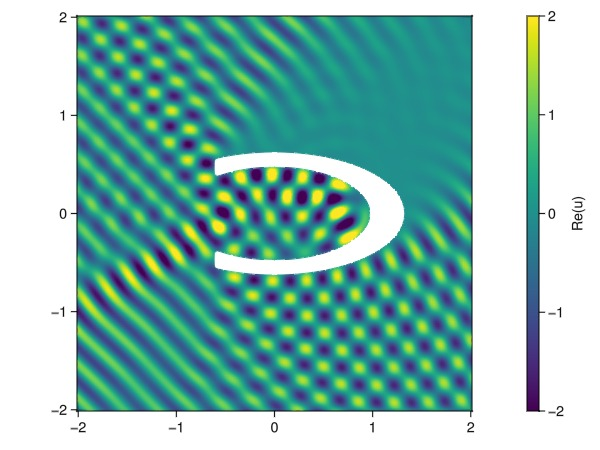
\includegraphics[width=0.5\linewidth]{images/cavity_fig.jpg}
    \caption{Geometry used in the test.}
    \label{fig:cavity_fig}
\end{figure}


We begin by running smaller examples and study the bounds found of \autoref{chap:gmres}, mainly \ref{eq:bound_E} and \ref{eq:boundE_final}. Satisfying these bounds is a guarantee that the residual measured at each k-th iteration, $\tilde{r_{k}}$, is close to the exact one $r_{k} =b-Ax_{k}$.

%FIXME: Expliquer le setup numerique: qu est ce qu'on met la et qu est ce que ça veut dire

This test run was executed with a smaller $A$, of dimensions $1650\times 1650$, and we use $\epsilon = 10^{-8}$ to assemble the hierarchical matrix as well as the algorithm's overall tolerance, i.e., the iterations stop as soon as $\frac{\norm{b - Ax_{k}}}{\norm{b}} \leq \epsilon$. The plots are in \autoref{fig:bound44}.

\begin{figure}[h!]
    \centering
    \begin{subfigure}[b]{0.5\linewidth}
        \includesvg[width=\linewidth]{images/bound_study.svg}
        %\label{fig:bound44_norm}
        \caption{Evolution for the upper bound of $||E_{k}||$, using $\ell_{k}=1$ and $\ell_{k}=\frac{\sigma_{k}(H_{k})}{k}$.}
    \end{subfigure}

    \begin{subfigure}[b]{0.3\linewidth}
        \includesvg[width=\linewidth]{images/bounds_44_normal.svg}
        %\label{fig:bound44_norm}
        \caption{Evolution of the upper bound in $\norm{r_{k} - \tilde{r_{k}}}$ for the case $\ell_{k}=1$.}
    \end{subfigure}
    \begin{subfigure}[b]{0.3\linewidth}
        \includesvg[width=\linewidth]{images/bounds_44_sing.svg}
        %\label{fig:bound44_sing}
        \caption{Evolution of the upper bound in $\norm{r_{k} - \tilde{r_{k}}}$ for the case $\ell_{k}=\frac{\sigma_{k}(H_{k})}{k}$.}
    \end{subfigure}
    \caption{Upper bound study for the perturbation and residuals involved in the cavity scattering problem. The hierarchical matrix was assembled with a $10^{-8}$ tolerance.}
    \label{fig:bound44}
\end{figure}

The bigger picture in \autoref{fig:bound44} shows how the different bounds of the perturbation's behave through iterations. Recalling that a greater tolerance means a bigger room to work with larger perturbations of $A$, what can make the inexact matrix-vector product faster.

The plot shows choosing $\ell_{k} = 1$, what makes the inexact product's tolerance bigger, i.e., “allows” for a more perturbed $A$, still respects the restriction in the bound \ref{eq:borne_delta}, as we can see on the left smaller plot. This shows bigger tolerances can still be used to achieve higher acceleration, while still maintaining the residual in a proper value. The different heuristics for the product tolerances at each iteration did not result in big variations in the total amount of iterations for the Inexact GMRES.

Passing on to the speed-up evaluation, we repeat a similar numeral setup: $A$ is assembled using the overall tolerance $\epsilon = 10^{-8}$. All product tolerances for each iteration, $\nu_{k}$, are obtained through the heuristic in \ref{eq:gen_heuristics}. We fix $A$'s dimensions as a $40000\times 40000$ matrix, and change the overall tolerance passed to the algorithm, varying from $10^{-8}$ to $10^{-2}$. The speed-up results for this fixed size test, as well as their respective relative residuals, are in \autoref{fig:cavity_results}.

\begin{figure}[h!]
    \centering
    \begin{subfigure}[b]{0.6\linewidth}
        \includesvg[width=\linewidth]{images/cavity_fixsize_speedup.svg}
        \caption{Speed-up measured for the fixed size cavity scattering problem.}
    \end{subfigure}
    \begin{subfigure}[b]{0.4\linewidth}
        \includesvg[width=\linewidth]{images/cavity_fixsize_residual.svg}
        \caption{Relative residual measured for the fixed size cavity scattering problem.}
    \end{subfigure}
    \begin{subfigure}[b]{0.4\linewidth}
        \includesvg[width=\linewidth]{images/cavity_fixsize_iterations.svg}
        \caption{Number of iterations for the fixed size cavity scattering problem.}
    \end{subfigure}
    \caption{Speed-up, relative residual and amount of iterations results for the Inexact GMRES algorithm in the cavity scattering problem. The hierarchical matrix $A$ was assembled with $10^{-8}$ tolerance and had a fixed $40000 \times 40000$ size.}
    \label{fig:cavity_results}
\end{figure}

As we can see, the speed-up did not cause a worse relative residual for the solution, always keeping it under the overall tolerance $\epsilon$ given for the algorithm. But, we can see the existence of a trade-off between tolerance and speed-up: lower precision in the algorithm may lead to a slower execution. The different number of iterations needed for each run, also in \autoref{fig:cavity_results}, shows that the slower results in the lower tolerance rate are not result of a larger number iterations, but maybe heavier ones in comparison to the exact algorithm.

For the last numerical setup, we again assemble $A$ with $10^{-8}$ tolerance, but now its dimensions will change while keeping the overall tolerance passed to the algorithm, $\epsilon$, fixed at $10^{-4}$.

\begin{figure}[h!]
    \centering
    \begin{subfigure}[b]{0.6\linewidth}
        \includesvg[width=\linewidth]{images/cavity_fixtol_speedup.svg}
        \caption{Speed-up measured for the fixed tolerance cavity scattering problem.}
    \end{subfigure}
    \begin{subfigure}[b]{0.4\linewidth}
        \includesvg[width=\linewidth]{images/cavity_fixtol_residual.svg}
        \caption{Relative residual for the fixed tolerance cavity scattering problem.}
    \end{subfigure}
    \begin{subfigure}[b]{0.4\linewidth}
        \includesvg[width=\linewidth]{images/cavity_fixtol_iterations.svg}
        \caption{Number of iterations for the fixed tolerance cavity scattering problem.}
    \end{subfigure}
    \caption{Speed-up, relative residual and amount of iterations results for the Inexact GMRES algorithm in the cavity scattering problem. The hierarchical matrix $A$ was assembled with $10^{-8}$ tolerance and used a overall tolerance $\epsilon = 10^{-4}$ to the algorithm.}
    \label{fig:cavity_resultsfixtol}
\end{figure}


\cleardoublepage % coloca o número de página correto das referências bibliográficas no sumário
\phantomsection % faz o link para a página correta das referências bibliográficas

%\addcontentsline{toc}{chapter}{References}
\bibliography{bibliografia}
\bibliographystyle{plain}
\nocite{*}

%\include{Sections/A-Apendix}

\end{document}
